\documentclass{article}

\usepackage{tikz}

\begin{document}
\begin{figure}
\begin{tikzpicture}[node distance=2in]
%\node(a) at (0,0) {a};
%\node(b) at (1,0) {b};
%\node(Fa) at (0,-1){F a};
%\node(Fb) at (1,-1){F b};
\node(xs0) {raw data};
\node(xs1) [below of=xs0] {processed data};
\node(m0) [right of=xs0] {raw model};
\node(m1) [right of=xs1] {processed model};

\draw[->] (xs0) to (xs1);
\draw[->] (xs0) to (m0);
\draw[->] (xs1) to (m1);
\draw[->] (m0) to (m1);
\end{tikzpicture}
\end{figure}


\begin{figure}
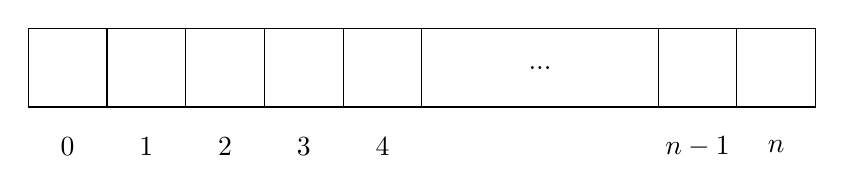
\begin{tikzpicture}
\node[minimum size=1cm,draw] at (0,0) {};
\node[minimum size=1cm,draw] at (1,0) {};
\node[minimum size=1cm,draw] at (2,0) {};
\node[minimum size=1cm,draw] at (3,0) {};
\node[minimum size=1cm,draw] at (4,0) {};
\node[minimum size=1cm,minimum width=3cm,draw] at (6,0) {...};
\node[minimum size=1cm,draw] at (8,0) {};
\node[minimum size=1cm,draw] at (9,0) {};

\node at (0,-1) {0};
\node at (1,-1) {1};
\node at (2,-1) {2};
\node at (3,-1) {3};
\node at (4,-1) {4};
\node at (8,-1) {$n-1$};
\node at (9,-1) {$n$};
\end{tikzpicture}
\end{figure}

\begin{figure}
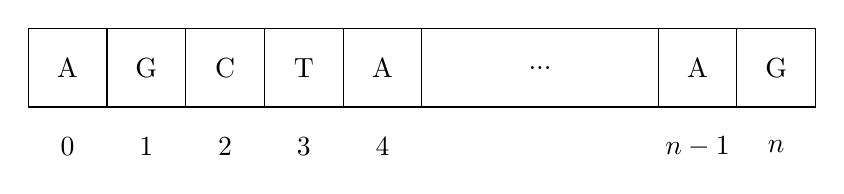
\begin{tikzpicture}
\node[minimum size=1cm,draw] at (0,0) {A};
\node[minimum size=1cm,draw] at (1,0) {G};
\node[minimum size=1cm,draw] at (2,0) {C};
\node[minimum size=1cm,draw] at (3,0) {T};
\node[minimum size=1cm,draw] at (4,0) {A};
\node[minimum size=1cm,minimum width=3cm,draw] at (6,0) {...};
\node[minimum size=1cm,draw] at (8,0) {A};
\node[minimum size=1cm,draw] at (9,0) {G};

\node at (0,-1) {0};
\node at (1,-1) {1};
\node at (2,-1) {2};
\node at (3,-1) {3};
\node at (4,-1) {4};
\node at (8,-1) {$n-1$};
\node at (9,-1) {$n$};
\end{tikzpicture}
\end{figure}

\end{document}
